\documentclass[border=10pt]{standalone}
\usepackage{tikz}
\usetikzlibrary{arrows.meta, shapes, calc}

\begin{document}
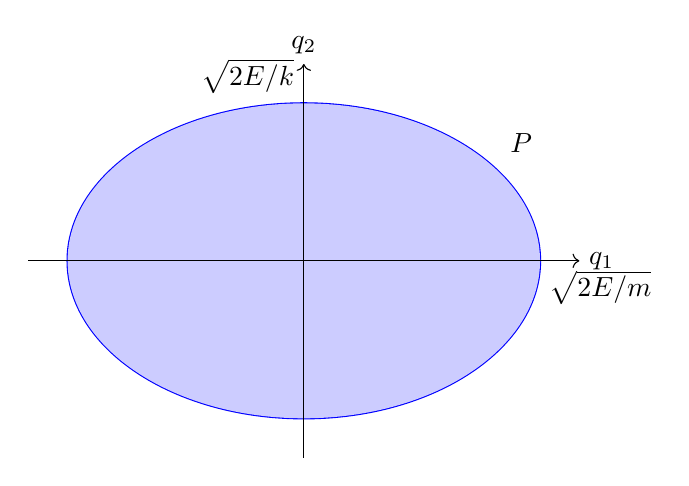
\begin{tikzpicture}
    % Draw the ellipse
    \draw[thick, blue] (0,0) ellipse (3cm and 2cm);
    
    % Shade the ellipse
    \fill[blue!20] (0,0) ellipse (3cm and 2cm);
    
    % Draw the coordinate axes
    \draw[->] (-3.5,0) -- (3.5,0) node[right] {$q_1$};
    \draw[->] (0,-2.5) -- (0,2.5) node[above] {$q_2$};
    
    % Label the intersection points
    \node at (3,0) [below right] {$\sqrt{2E/m}$};
    \node at (0,2) [above left] {$\sqrt{2E/k}$};
    
    % Label the point P
    \node at (2.5,1.5) [right] {$P$};
\end{tikzpicture}
\end{document}